\def\layersep{3cm}
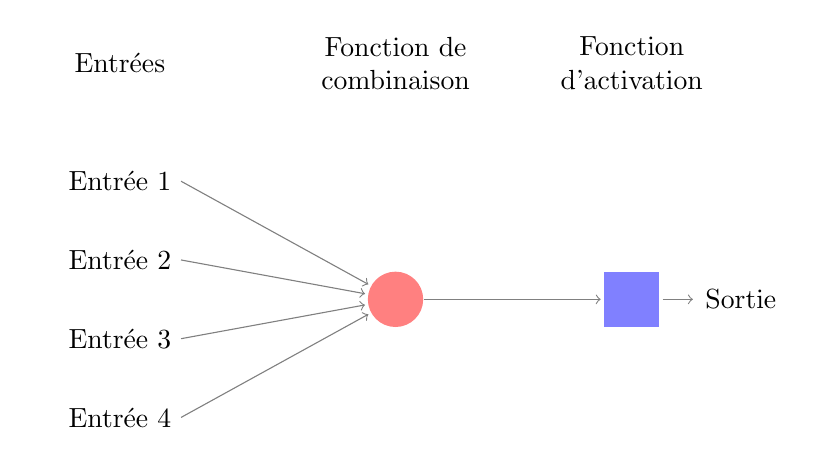
\begin{tikzpicture}[shorten >=1pt,->,draw=black!50, node distance=\layersep]
    \tikzstyle{every pin edge}=[<-,shorten <=1pt]
    \tikzstyle{input}=[rectangle];
    \tikzstyle{output neuron}=[circle,minimum size=20pt, fill=red!50];
    \tikzstyle{nonlinearity}=[rectangle,minimum size=20pt, fill=blue!50];
    \tikzstyle{annot} = [text width=6em, text centered]

    % Draw the input layer nodes
    \foreach \name / \y in {1,...,4}
    % This is the same as writing \foreach \name / \y in {1/1,2/2,3/3,4/4}
        \node[input] (I-\name) at (0,-\y) {Entr\'{e}e \y};

    % Draw the output layer node
    \node[output neuron, right of=I-1,xshift=-.5cm] (Syn) at (,-2.5) {};
    % Draw the output layer node
    \node[nonlinearity,pin={[pin edge={->}]right:Sortie}, right of=Syn] (NL) {};

    % Connect every node in the input layer with every node in the
    % hidden layer.
    \foreach \source in {1,...,4}
        \path (I-\source.east) edge (Syn);
	\path (Syn) edge (NL);

    % Annotate the layers
    \node[annot,above of=I-1, node distance=1.5cm] (hl) {Entr\'{e}es};
    \node[annot,above of=Syn] (hl) {Fonction de combinaison};
    \node[annot,above of=NL] (hl) {Fonction d'activation};
\end{tikzpicture}